\documentclass[journal,11pt,onecolumn,draftclsnofoot]{IEEEtran}
% Note: To compile as standard two-column camera-ready journal, replace above with:
% \documentclass[journal]{IEEEtran}

\usepackage{cite}
\usepackage{amsmath,amssymb,amsfonts}
\usepackage{mathtools}
\usepackage{graphicx}
\usepackage{xcolor}
\usepackage{booktabs}
\usepackage{array}
\usepackage{multirow}
\usepackage{tabularx}
\usepackage{url}
\usepackage{microtype}
\usepackage[hidelinks]{hyperref}

\newcommand{\GS}{\textsc{gs}}
\newcommand{\WL}{\textsc{wl}}
\graphicspath{{figs/}}

\begin{document}

\title{Replication and Quality-Gated Extension of Automated Weak Supervision for Label-Scarce Medical Image Segmentation}

\author{\IEEEauthorblockN{Vijay Aditya R\,V\IEEEauthorrefmark{1},
Harini N\IEEEauthorrefmark{1}, and
Regella Krishna Saketh\IEEEauthorrefmark{1}}
\IEEEauthorblockA{\IEEEauthorrefmark{1}Department of Computer Science and Engineering\\
Emails: vijayadityarv@gmail.com, harinin006@gmail.com, krishnasaketh566@gmail.com}}

\maketitle

%==============================================================================
\begin{abstract}
Annotating medical scans at the pixel level demands specialized clinician time, rendering training datasets in clinical environments inherently constrained. Foundation architectures such as the Segment Anything Model (SAM) and its domain-specific derivative MedSAM offer promptable zero-shot delineations, but require accurate spatial prompts to prevent catastrophic over- or under-segmentation. Deshpande et al.\ (MIDL 2024) addressed this challenge through Auto-Generate-WLs, a workflow that initializes a compact segmentor on limited gold-standard annotations ($\le 25$ cases) to automatically synthesize prompt coordinates for MedSAM, producing weak masks to expand the training distribution. 

In this work, we present an empirical replication of this pipeline alongside an examination of multi-stage quality filtration. Across breast ultrasonography (BUSI), dermoscopic lesion analysis (ISIC 2018), and chest radiography, we benchmark replication fidelity and investigate five modular enhancements: (i)~a sequential five-tier quality cascade combining textural complexity classification, rotational invariance checks, boundary refinement, morphological gating, and gradient-boosted radiomics quality estimation; (ii)~curriculum-guided easy-first sample scheduling; (iii)~a contour-distance-attenuated retraining loss; (iv)~self-supervised contrastive representation pretraining; and (v)~multi-perspective test-time augmentation (TTA). 

Empirically, our reproduction of the 100-weak-label bounding-box configuration on BUSI attains a test Dice coefficient of 0.4631, closely matching the published 0.4661 baseline. Replicating point-based prompting on BUSI yields a Dice score of 0.6111, exceeding the published mark of 0.5302. However, our multi-stage quality cascade exhibits extreme selectivity, passing only 33 of 493 candidate ultrasound scans (6.7\%) and 6 of 200 dermoscopy candidates (3.0\%). Under the repository's native evaluation routine, models retrained on these sparse, filtered cohorts fall short of baseline gold-standard benchmarks (BUSI: 0.3905 vs.\ 0.4209; ISIC 2018: 0.6149 vs.\ 0.6779). Under an alternative evaluation routine, the enhanced BUSI network records 0.3966 compared to 0.3846 for the baseline, with flip-based inference yielding modest within-script gains (+0.001 to +0.019 Dice). Self-supervised contrastive pretraining minimized latent NT-Xent loss reliably (0.7060 to 0.5020 on BUSI; 4.1071 to 3.6013 on ISIC), although representations were isolated from downstream retraining. We report cell-indexed metric provenance across all executed notebooks and discuss the trade-off between pseudo-mask selectivity and supervisory data volume.
\end{abstract}

\begin{IEEEkeywords}
Medical image segmentation, label scarcity, MedSAM, vision foundation models, weak supervision, quality control, contrastive learning, test-time augmentation, reproducibility.
\end{IEEEkeywords}

%==============================================================================
\section{Introduction}
\label{sec:intro}

\IEEEPARstart{P}{recise} pixel-level delineation of pathological margins—such as solid breast tumors in sonography, melanocytic lesions in dermoscopy, and pleural air collections in chest radiography—serves as the cornerstone of computer-assisted clinical diagnostics and radiation therapy planning~\cite{tajbakhsh2020}. Contemporary deep convolutional architectures, most notably UNet++~\cite{zhou2018}, yield robust delineations when parameterized on extensive corpora of expert annotations. Nonetheless, manual pixel-level annotation requires significant radiologist and pathologist time, generating substantial labeling cost and inter-observer variability~\cite{tajbakhsh2020}. In emerging clinical scenarios, practitioners routinely confront acute \emph{label scarcity}, where only 20 to 50 verified ground-truth cases can be obtained, despite the presence of hundreds of unannotated imaging studies.

The emergence of vision foundation models, most notably the Segment Anything Model (SAM)~\cite{kirillov2023} and its clinical counterpart MedSAM~\cite{ma2023medsam}, has reshaped interactive computer vision. Fine-tuned over 1.5 million radiological and histological pairs across 15 anatomical domains, MedSAM achieves strong zero-shot segmentation when supplied with accurate prompt coordinates~\cite{ma2023medsam}. However, foundation models remain inherently interactive prompt followers rather than fully autonomous target detectors. In the absence of manual coordinates, autonomous grid prompting in SAM yields severe over-fragmentation, while MedSAM collapses into blank or degenerate prediction masks~\cite{deshpande2024}. Moreover, slight spatial offsets in prompt boundaries cause foundation models to bleed into surrounding healthy tissue or truncate lesion margins~\cite{deoliveira2023,he2023sam}.

To resolve manual prompt dependency, Deshpande et al.~\cite{deshpande2024} (MIDL 2024) formulated the Auto-Generate-WLs pipeline. In their schema, an initial lightweight UNet++ is fitted to a minimal gold-standard (GS) seed set ($N \le 25$). The coarse segmentation outputs produced across the unlabeled pool are converted into automated bounding boxes or point clicks, prompting MedSAM to synthesize pseudo-labels. The segmentor is subsequently retrained on the pooled corpus. Relying only on a coarse filter that eliminates masks with greater than 97\% uniform background or foreground area, the authors reported substantial empirical gains across breast ultrasound (BUSI), dermoscopy (ISIC), and chest radiography (CANDID-PTX)~\cite{deshpande2024}.

In this work, we conduct a two-part empirical study:
\begin{enumerate}
    \item \textbf{Empirical Replication:} We reproduce the foundation weak-labeling pipeline on breast ultrasound, dermoscopy, and thoracic radiographs, auditing training hyperparameters, optimization dynamics, and test scores against published benchmarks.
    \item \textbf{Exploration of Modular Quality Control:} We formulate and implement a multi-stage quality verification suite—incorporating complexity classification, multi-angle transformation consistency, morphological filtering, radiomics quality estimation, curriculum sorting, distance-weighted loss reweighting, and test-time augmentation (TTA)—to determine whether automated quality checks improve downstream segmentor performance.
\end{enumerate}

Our findings contribute critical observations to the medical image computing community. Replicating the 100-weak-label regime on BUSI closely mirrors the published box-prompt benchmark (0.4631 replicated vs.\ 0.4661 published) and exceeds the point-prompt benchmark (0.6111 vs.\ 0.5302). Conversely, our five-stage quality cascade proved exceptionally strict, rejecting over 93\% of ultrasound scans and 97\% of dermoscopy scans. Retraining on these minimal, highly filtered sets yielded lower scores than baseline models under standard evaluation scripts. We report cell-indexed provenance for every metric, discuss the trade-off between weak-label purity and sample volume, and identify procedural factors relevant to practical deployment.

%==============================================================================
\section{Related Work}
\label{sec:related}

\subsection{Supervision Under Extreme Annotation Scarcity}
Semi-supervised learning (SSL) seeks to extract supervisory signals from unannotated clinical scans. Established strategies encompass confidence-thresholded self-training~\cite{lee2013}, mean-teacher parameter ensembling~\cite{tarvainen2017}, uncertainty-guided consistency regularization~\cite{yu2019}, and cross-pseudo supervision between dual backbones~\cite{chen2021cps}. Self-supervised contrastive learning~\cite{chen2020simclr,chaitanya2020} maps raw scans into semantically organized embedding spaces prior to few-shot supervised tuning. In-context models like UniverSeg~\cite{butoi2023} delineate query targets via cross-attention with support exemplars without gradient descent updates. The Auto-Generate-WLs framework~\cite{deshpande2024} diverges from conventional self-training: pseudo-masks originate not from the network's own uncalibrated logits, but from a decoupled, frozen medical foundation model (MedSAM) prompted by the primary network.

\subsection{Domain Adaptation of Foundation Segmentors}
SAM~\cite{kirillov2023} employs a heavy Vision Transformer image encoder coupled with prompt tokens and a lightweight decoder. While effective on natural scenes, direct zero-shot evaluation on clinical modalities exposes severe degradation from imaging artifacts and speckle noise~\cite{deoliveira2023,he2023sam}. MedSAM~\cite{ma2023medsam} bridges this domain divide via large-scale medical pretraining. Dedicated adaptations include SAMUS for sonography~\cite{lin2023}, CEmb-SAM for heterogeneous multi-center datasets~\cite{shin2023}, and MA-SAM for 3D volumetric scans~\cite{chen2023}. Automated prompting mechanisms have been explored using auxiliary detectors such as YOLOv8~\cite{pandey2023}, template cross-correlation~\cite{anand2023}, and extreme-point localization~\cite{lei2023}. The baseline method~\cite{deshpande2024} extracts prompt coordinates directly from coarse segmentor outputs; our study extends this approach by evaluating multi-tiered post-generation verification.

\subsection{Test-Time Augmentation and Inference Stability}
Test-time augmentation (TTA)—averaging model inferences over spatial reflections and rotations of an input image—provides post-hoc variance reduction and aleatoric uncertainty estimation in medical computer vision~\cite{wang2019}. Because TTA requires no parameter retraining, it operates as an inference-time ensembling device across trained checkpoints.

%==============================================================================
\section{Background and Problem Formulation}
\label{sec:background}

\subsection{Mathematical Formulation and Metrics}
\label{subsec:metrics}
Let $\mathcal{X} \subset \mathbb{R}^{H \times W \times C}$ denote the input scan domain, and let $\mathcal{Y} \subset \{0, 1\}^{H \times W}$ represent the binary target space. Under extreme label scarcity, the clinical dataset is partitioned into three disjoint subsets:
\begin{enumerate}
    \item \textbf{Gold-Standard Set:} $\mathcal{D}_{\text{labeled}} = \{(x_i, y_i^*)\}_{i=1}^{N_L}$, where $N_L \in [20, 25]$ represents expert manual annotations.
    \item \textbf{Unlabeled Pool:} $\mathcal{D}_{\text{unlabeled}} = \{x_j\}_{j=1}^{N_U}$, where $N_U \gg N_L$ (typically $N_U \in [200, 500]$).
    \item \textbf{Locked Evaluation Partition:} $\mathcal{D}_{\text{test}} = \{(x_k, y_k^*)\}_{k=1}^{N_T}$, strictly reserved for performance reporting.
\end{enumerate}

For a predicted mask $P \in \{0, 1\}^{H \times W}$ and ground truth $G \in \{0, 1\}^{H \times W}$, the Dice Similarity Coefficient and Intersection over Union (IoU / Jaccard Index) are formulated as:
\begin{equation}
\mathrm{Dice}(P, G) = \frac{2|P \cap G|}{|P| + |G|}, \qquad \mathrm{IoU}(P, G) = \frac{|P \cap G|}{|P \cup G|}.
\label{eq:metrics}
\end{equation}
At the individual scan level, the algebraic identity $\mathrm{Dice} = \frac{2\,\mathrm{IoU}}{1+\mathrm{IoU}}$ mandates that $\mathrm{Dice} \ge \mathrm{IoU}$. Across multi-image test sets, aggregation protocols differ substantially:
\begin{itemize}
    \item \emph{Macro-Averaging (Image-Wise Mean):} $\overline{\mathrm{Dice}}_{\text{macro}} = \frac{1}{N_T}\sum_k \mathrm{Dice}(P_k, G_k)$, assigning uniform importance to every scan.
    \item \emph{Micro-Averaging (Dataset Pooled Ratio):} $\overline{\mathrm{Dice}}_{\text{micro}} = \frac{2\sum_k |P_k \cap G_k|}{\sum_k (|P_k| + |G_k|)}$, which is dominated by scans with large anatomical targets.
\end{itemize}
When small lesions are poorly delineated while large structures are accurately captured, micro-averaged IoU can numerically exceed macro-averaged Dice. Maintaining uniform script protocols is therefore essential for rigorous model ranking.

\subsection{MedSAM Architecture and Prompt Dynamics}
MedSAM~\cite{ma2023medsam} encodes an input scan resized to $1024 \times 1024$ through a Vision Transformer (ViT-B) backbone. The prompt encoder projects bounding box corners $[x_1, y_1, x_2, y_2]$ or point coordinates into 256-dimensional tokens. The mask decoder applies two-way cross-attention between image embeddings and prompt tokens, producing continuous logit maps thresholded at $0.5$. The synthesized mask depends heavily on prompt dimensions: oversized boxes incorporate adjacent non-target tissue, whereas overly narrow boxes cause lesion truncation~\cite{deshpande2024}. Autonomous unprompted execution produces blank segmentations, mandating external prompt synthesis.

\subsection{Prompt Synthesis and the 97\% Area Rule}
Given coarse probability maps from UNet++, the base method~\cite{deshpande2024} discards empty predictions, extracts the largest connected component, and removes small peripheral fragments. For bounding-box prompting, the extreme coordinate indices of the component define the prompt window. For point prompting, the centroid of the primary component serves as a positive prompt, while background coordinates with coarse confidence below $0.1$ serve as negative prompts. The only filtering step in~\cite{deshpande2024} eliminates weak masks where background or foreground occupies more than 97\% of the image area.

\subsection{Supervised Training Objective}
UNet++~\cite{zhou2018} is trained minimizing a compound objective:
\begin{equation}
\mathcal{L}_{\text{base}} = \mathcal{L}_{\text{Dice}}(\hat{y}, y) + 0.5\,\mathcal{L}_{\text{BCE}}(\hat{y}, y),
\label{eq:baseloss}
\end{equation}
where $\mathcal{L}_{\text{Dice}} = 1 - \frac{2\sum_p \hat{y}_p y_p + \epsilon}{\sum_p \hat{y}_p + \sum_p y_p + \epsilon}$ and $\mathcal{L}_{\text{BCE}}$ denotes binary cross-entropy.

\subsection{Published Reference Benchmarks}
\label{subsec:pubabl}
Table~\ref{tab:pubabl} summarizes reference ablations reported in~\cite{deshpande2024}. These comprise synthetic image generation via Denoising Diffusion Probabilistic Models (DDPM)~\cite{ho2020,wolleb2021} and retinal vessel segmentation on CHASE~\cite{fraz2012}, where adding weak supervision failed to yield improvements.

\begin{table}[t]
\renewcommand{\arraystretch}{1.12}
\caption{Reference Ablations Published in Deshpande et al.~\cite{deshpande2024} (Not Replicated Locally)}
\label{tab:pubabl}
\centering\scriptsize\setlength{\tabcolsep}{4pt}
\begin{tabular}{@{}llcccc@{}}
\toprule
\multicolumn{6}{@{}l}{\textit{BUSI Label Scarcity Ablation (Synthetic Weak Labels)}} \\
GS Labels & 10 & 25 & 50 & 100 & --- \\
GS Only & 0.2327 & 0.3059 & 0.4379 & 0.5575 & --- \\
GS + 100 WL & 0.2637 & 0.4661 & 0.5416 & 0.6155 & --- \\
\midrule
\multicolumn{6}{@{}l}{\textit{BUSI SAM vs.\ MedSAM Comparison (25 GS + 100 WL)}} \\
Baseline GS & SAM Auto & MedSAM Auto & SAM Prompted & MedSAM Prompted & --- \\
0.3059 & 0.2124 & 0.0000 & 0.3886 & 0.4661 & --- \\
\midrule
\multicolumn{6}{@{}l}{\textit{Synthetic Data Experiments (25 GS; Weak Labels: 50 / 250 / 500)}} \\
Dataset & 0 WL & 50 WL & 250 WL & 500 WL & --- \\
BUSI & 0.3059 & 0.4177 & 0.4312 & 0.4301 & --- \\
ISIC & 0.6123 & 0.7762 & 0.7228 & 0.7247 & --- \\
CANDID-PTX & 0.8182 & 0.8997 & 0.9073 & 0.9022 & --- \\
\midrule
\multicolumn{6}{@{}l}{\textit{CHASE Retinal Vessel Segmentation (5 GS; Weak Labels: 0 / 5 / 10 / 15)}} \\
Weak Labels & 0 & 5 & 10 & 15 & --- \\
Dice & 0.2406 & 0.2557 & 0.2180 & 0.2081 & --- \\
\bottomrule
\end{tabular}
\end{table}

%==============================================================================
\section{Replicated Baseline and Proposed Additions}
\label{sec:method}

\subsection{Baseline Replication Workflow}
The replicated baseline adheres to the published protocol~\cite{deshpande2024}:
\begin{enumerate}
    \item Train UNet++ on $\mathcal{D}_{\text{GS}}$ ($N=25$) minimizing~\eqref{eq:baseloss}.
    \item Predict coarse probability masks across unannotated scans $\mathcal{D}_{\text{U}}$.
    \item Extract the primary connected component and compute bounding box limits.
    \item Query MedSAM (ViT-B) to synthesize candidate weak labels $\tilde{Y}$.
    \item Exclude degenerate masks exceeding the 97\% uniform area rule.
    \item Retrain UNet++ on the augmented collection $\mathcal{D}_{\text{GS}} \cup \mathcal{D}_{\text{WL}}$.
\end{enumerate}

Table~\ref{tab:setup} compares hyperparameter configurations between the published study and our execution.

\begin{table}[t]
\renewcommand{\arraystretch}{1.15}
\caption{Hyperparameter Comparison: Published Study~\cite{deshpande2024} vs.\ Our Replication}
\label{tab:setup}
\centering\footnotesize
\begin{tabular}{@{}lll@{}}
\toprule
Hyperparameter & Published Setting~\cite{deshpande2024} & Our Experimental Setting \\
\midrule
Network Backbone & UNet++ & UNet++ (NestedUNet) \\
Optimizer & SGD (momentum 0.9) & Adam ($\beta_1=0.9, \beta_2=0.999$) \\
Learning Rate & $1 \times 10^{-3}$ & $3 \times 10^{-4}$ \\
Scheduler & Cosine Annealing ($\min = 10^{-5}$) & Cosine Annealing ($\min = 10^{-5}$) \\
Loss Function & Dice + 0.5 BCE & Repository \texttt{BCEDiceLoss} \\
Epoch Budget & 100 epochs & 200 epochs \\
Batch Size / Resolution & 4 / $256 \times 256$ & 4 / $256 \times 256$ \\
Random Seed & Not specified & Seed 42 (deterministic) \\
Hardware & NVIDIA RTX A4000 & Google Colab GPU (T4 / A100) \\
\bottomrule
\end{tabular}
\end{table}

\begin{figure*}[t]
\centering
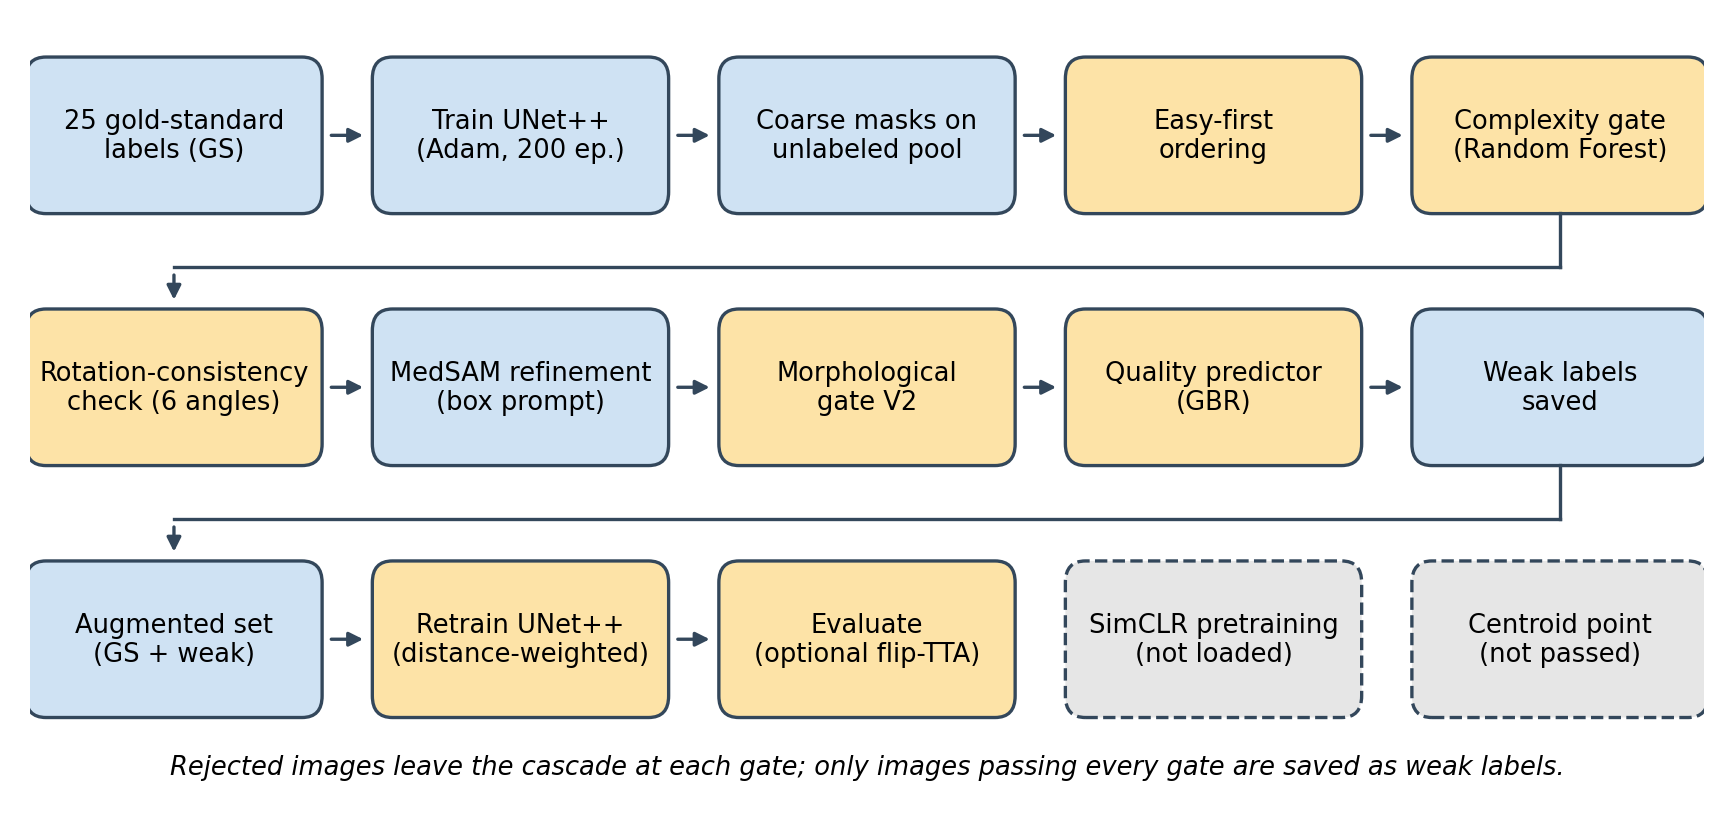
\includegraphics[width=0.92\textwidth]{fig1_pipeline.png}
\caption{Architectural overview of the weak-label generation pipeline and evaluated additions. Blue nodes indicate published steps from Deshpande et al.~\cite{deshpande2024}. Amber nodes indicate our evaluated quality additions connected to trained models. Grey dashed nodes represent isolated experimental modules.}
\label{fig:pipeline}
\end{figure*}

\subsection{Proposed Methodological Additions}
Fig.~\ref{fig:pipeline} outlines the positioning of each evaluated component. Table~\ref{tab:audit} provides a component-by-component status audit detailing execution, downstream connectivity, and isolation.

\subsubsection{Multi-Gate Quality Control Cascade}
Unlabeled scans are routed through a sequential five-stage quality cascade:
\begin{itemize}
    \item \textbf{Gate 1: Complexity Gating.} Image texture features (Canny edge density, Shannon entropy, mean intensity, variance, GLCM contrast, and energy) are extracted from each $256 \times 256$ grayscale scan. A Random Forest classifier (50 estimators) is trained on the 25 GS images to predict whether MedSAM refinement achieves $\mathrm{Dice} \ge 0.50$. An unlabeled scan is approved if predicted probability satisfies $\pi_{\text{comp}}(x) \ge \tau_{\text{comp}} = 0.15$. A fallback floor selects the top 40 scans if fewer qualify.
    \item \textbf{Gate 2: Rotational Transformation Consistency.} The scan is perturbed across six angular increments in $[-30^\circ, 30^\circ]$. The coarse network predicts on each view, masks are mapped back to native coordinates, and bounding boxes are extracted. The scan is approved if mean pairwise box IoU satisfies $\text{Cons}(x) \ge 0.20$.
    \item \textbf{Gate 3: MedSAM Prompt Refinement.} MedSAM is prompted with the bounding box of the primary connected component. Helper code computes centroid coordinates but executes MedSAM with \texttt{points=None}; bounding boxes were therefore used in all cascade runs.
    \item \textbf{Gate 4: Multi-Scale Morphological Gate.} Candidate masks are rejected if: (a) foreground area falls outside $[0.002, 0.97]$; (b) the secondary component ($\ge 50$ px) exceeds 0.75 of the primary component; (c) box aspect ratio exceeds 15.0; (d) convexity (mask area over convex hull area) is below 0.03; or (e) for dermoscopy, directional stripe ratio exceeds 7.0.
    \item \textbf{Gate 5: Radiomics Quality Estimation.} A Gradient Boosting Regressor (30 estimators) trained on the 25 GS scans estimates mask agreement using area, perimeter, eccentricity, intra-mask intensity, and GLCM contrast. Candidates with predicted score below $\tau_{\text{qual}} = 0.03$ are discarded.
\end{itemize}

\subsubsection{Curriculum Easy-First Scheduling}
Unlabeled scans are sorted by coarse prediction certainty ($\max_p \sigma(f(x))_p$ penalized by target area deviation). Scans are processed in descending order up to a cap of 100 weak labels.

\subsubsection{Boundary-Distance-Weighted Retraining Loss}
To account for boundary ambiguity in foundation-model segmentations, weak labels receive pixel weights derived from Euclidean distance $d(p)$ to the nearest mask contour $\partial M$:
\begin{equation}
w(p) = 0.4 + 0.6\,\frac{d(p)}{d_{\max}}.
\label{eq:dwl}
\end{equation}
Loss terms are scaled by sample factor $\lambda = 0.5$ for weak labels, whereas gold-standard samples retain uniform unit weights ($w=1.0, \lambda=1.0$):
\begin{equation}
\mathcal{L}_{\text{BCE}}^{w} = \frac{\lambda}{HW}\sum_p w(p)\,\mathrm{BCE}(\hat{y}_p, y_p), \qquad
\mathcal{L}_{\text{Dice}}^{w} = \lambda \left( 1 - \frac{2\sum_p w(p)\hat{y}_p y_p + \epsilon}{\sum_p w(p)\hat{y}_p + \sum_p w(p)y_p + \epsilon} \right).
\end{equation}

\subsubsection{SimCLR-Style Encoder Pretraining}
The UNet++ encoder is pretrained on unlabeled scans via the NT-Xent contrastive loss~\cite{chen2020simclr} across stochastic augmented views (15 epochs on BUSI; 5 epochs on ISIC). Checkpoint weights were saved to disk but were not imported into downstream segmentation training scripts (Table~\ref{tab:audit}).

\subsubsection{Dual-Perspective Test-Time Augmentation}
At inference, predictions are evaluated across horizontal reflection, vertical reflection, and compound reflections, projected back to native coordinates, and averaged before thresholding at $0.5$:
\begin{equation}
P_{\text{TTA}}(p) = \frac{1}{4}\left[ P(p) + P(p^h) + P(p^v) + P(p^{hv}) \right].
\label{eq:tta}
\end{equation}

\begin{table*}[t]
\renewcommand{\arraystretch}{1.12}
\caption{Systematic Audit of Experimental Components Against Notebook Implementations}
\label{tab:audit}
\centering\footnotesize
\begin{tabularx}{\textwidth}{@{}p{3.2cm}cccc X@{}}
\toprule
Component & Implemented & Executed & Reached Model & Isolated & Notebook Implementation Details \\
\midrule
Complexity Gate (RF) & Yes & BUSI, ISIC & Yes & No & Fitted to 25 GS scans; ISIC approval met fallback floor of 40. \\
Rotation Consistency & Yes & BUSI, ISIC & Yes & No & Primary rejector across modalities (82 BUSI, 20 ISIC). \\
Morphological Gate V2 & Yes & BUSI, ISIC & Yes & No & Removed 11 BUSI and 3 ISIC candidate masks. \\
Quality Regressor (GBR) & Yes & BUSI, ISIC & Yes & No & Cutoff 0.03; eliminated low-scoring boundary delineations. \\
Easy-First Ordering & Yes & BUSI, ISIC & No Effect & No & Weak-label cap was not reached; order did not alter saved set. \\
Centroid Prompting & Yes & Computed & No & No & Bounding boxes used in cascade (\texttt{points=None} passed to MedSAM). \\
Distance-Weighted Loss & Yes & BUSI, ISIC & Yes & No & Evaluated jointly with the cascade in retrained models. \\
SimCLR Pretraining & Yes & BUSI, ISIC & No & No & Loss logged; encoder weights not loaded into segmentation training. \\
Flip Test-Time Augmentation & Yes & BUSI, ISIC & Yes (BUSI) & Within Script & Evaluated via \texttt{eval\_tta.py}; metrics printed on BUSI. \\
SIIM-ACR Pipeline & Yes & Yes & No Output & --- & Pipeline coded in notebook; no evaluation output saved. \\
\bottomrule
\end{tabularx}
\end{table*}

%==============================================================================
\section{Datasets and Experimental Protocols}
\label{sec:data}

\subsection{Dataset Partitions}
Experiments evaluate three distinct medical imaging benchmarks (Table~\ref{tab:splits}):
\begin{itemize}
    \item \textbf{BUSI (Breast Ultrasound):}~\cite{aldhabyani2020} Comprises 647 benign and malignant lesion images with masks. An 80/20 partition produced a locked test set of 129 images, a gold-standard pool of 25 images, and an unannotated pool of 493 images with zero overlap.
    \item \textbf{ISIC 2018 (Dermoscopy):}~\cite{codella2019} Task 1 lesion segmentation data (2594 images) was partitioned into a locked test set of 518 images, 25 gold-standard images, and an unlabeled pool capped at 200 images for computational tractability. Because Deshpande et al.~\cite{deshpande2024} utilized the ISBI 2016 collection (1279 images)~\cite{gutman2016}, results are evaluated relative to our local baseline.
    \item \textbf{SIIM-ACR Pneumothorax:}\footnote{SIIM-ACR Pneumothorax Segmentation, Society for Imaging Informatics in Medicine and American College of Radiology, Kaggle, 2019.} Chest radiographs were prepared with 25 GS positives, an unlabeled pool of $\le 200$, and a 50-image test set. This targets pneumothorax boundaries, distinct from lung field segmentation in CANDID-PTX~\cite{feng2021}.
\end{itemize}

\begin{table}[t]
\renewcommand{\arraystretch}{1.15}
\caption{Dataset Partition Sizes Evaluated in Local Experiments}
\label{tab:splits}
\centering\footnotesize
\begin{tabular}{@{}lccccc@{}}
\toprule
Dataset & Modality & Total Scans & GS Pool ($N_L$) & Unlabeled Pool ($N_U$) & Test Set ($N_T$) \\
\midrule
BUSI & Breast Ultrasound & 647 & 25 & 493 & 129 \\
ISIC 2018 (Task 1) & Dermoscopy & 743 & 25 & 200 (capped) & 518 \\
SIIM-ACR (Positives) & Chest Radiographs & --- & 25 & $\le$200 & 50 \\
\bottomrule
\end{tabular}
\end{table}

\subsection{Evaluation Scripts and Verification Protocols}
Test metrics are documented using two independent scripts:
\begin{enumerate}
    \item \texttt{eval.py}: The repository's standard macro-averaging script.
    \item \texttt{eval\_tta.py}: A custom inference script supporting spatial transformations.
\end{enumerate}
All reported figures stem from deterministic single-seed runs (Seed 42) executed on Google Colab GPU hardware.

%==============================================================================
\section{Empirical Results}
\label{sec:results}

\subsection{Published Benchmark Reference Values}
Table~\ref{tab:published} documents the published reference results from Deshpande et al.~\cite{deshpande2024} for comparative perspective.

\begin{table}[t]
\renewcommand{\arraystretch}{1.15}
\caption{Published Dice Scores from Deshpande et al.~\cite{deshpande2024} (Reference Only)}
\label{tab:published}
\centering\footnotesize
\begin{tabular}{@{}lcccc@{}}
\toprule
Configuration & Prompt Type & BUSI & ISIC & CANDID-PTX \\
\midrule
UniverSeg (Few-Shot)~\cite{butoi2023} & Support Exemplars & 0.3681 & 0.5257 & 0.7700 \\
SAM (Autonomous Grid)~\cite{kirillov2023} & Automatic & 0.2124 & 0.5893 & 0.4115 \\
\midrule
25 GS Baseline (0 WL) & --- & 0.3059 & 0.6123 & 0.8182 \\
25 GS + 100 WL & Bounding Box & 0.4661 & 0.7424 & \textbf{0.9096} \\
25 GS + 100 WL & Points Prompt & \textbf{0.5302} & \textbf{0.8483} & 0.8443 \\
\bottomrule
\end{tabular}
\end{table}

\subsection{Empirical Results on Breast Ultrasound (BUSI)}
Table~\ref{tab:busi} and Fig.~\ref{fig:results} record empirical performance across the 129-image BUSI test set using \texttt{eval.py}.

\begin{table}[t]
\renewcommand{\arraystretch}{1.15}
\caption{BUSI Test Set Performance (\texttt{eval.py}, 129 Test Images, Seed 42)}
\label{tab:busi}
\centering\footnotesize
\begin{tabular}{@{}lcc@{}}
\toprule
Model Configuration & IoU & Dice \\
\midrule
GS Baseline (20 Train / 5 Val of 25 GS) & 0.3571 & 0.4209 \\
Enhanced Model (20 GS + 33 Cascade WL, DW Loss) & 0.2853 & 0.3905 \\
Replicated Set (25 GS + 100 WL, Box Prompts) & 0.3266 & 0.4631 \\
Replicated Set (25 GS + 100 WL, Point Prompts) & \textbf{0.4732} & \textbf{0.6111} \\
\bottomrule
\end{tabular}
\end{table}

\begin{figure*}[t]
\centering
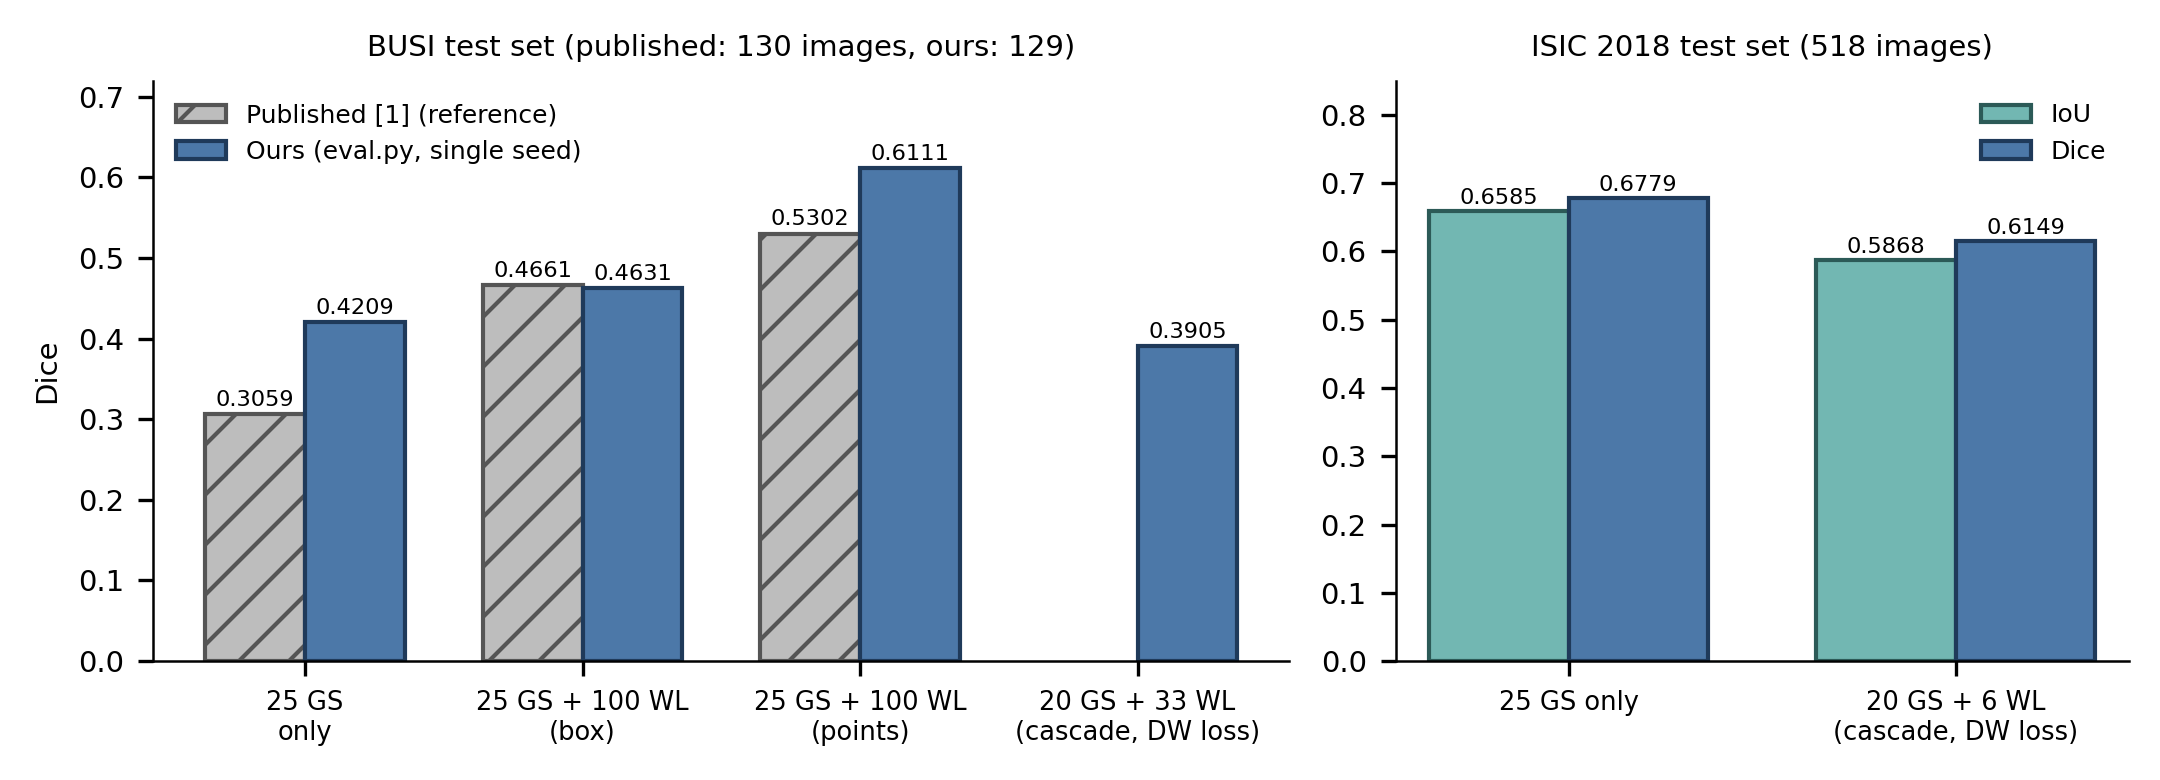
\includegraphics[width=0.92\textwidth]{fig2_results.png}
\caption{Empirical segmentation scores on locked test sets. Left: BUSI Dice from \texttt{eval.py}; hatched bars denote published values~\cite{deshpande2024} for reference. Right: ISIC 2018 IoU and Dice for the GS baseline and enhanced cascade model.}
\label{fig:results}
\end{figure*}

\subsection{Replication Fidelity on BUSI}
Table~\ref{tab:repl} contrasts reproduced configurations against published values:
\begin{itemize}
    \item \textbf{Bounding-Box Replication:} Retraining on 25 GS + 100 WL with bounding boxes reached 0.4631 Dice, replicating the published 0.4661 within an absolute deviation of $-0.0030$.
    \item \textbf{Point-Prompt Replication:} Retraining on 25 GS + 100 WL with point prompts achieved 0.6111 Dice, exceeding the published 0.5302 benchmark by $+0.0809$ Dice ($+15.3\%$ relative gain).
    \item \textbf{Baseline Discrepancy:} Our 25 GS baseline yielded 0.4209 Dice (vs.\ 0.3059 published), attributable to optimizer selection (Adam vs.\ SGD) and training budget (200 vs.\ 100 epochs).
\end{itemize}

\begin{table}[t]
\renewcommand{\arraystretch}{1.15}
\caption{Replication Fidelity: Published vs.\ Replicated Dice Scores on BUSI}
\label{tab:repl}
\centering\footnotesize
\begin{tabular}{@{}lccc@{}}
\toprule
Configuration & Published~\cite{deshpande2024} & Ours (\texttt{eval.py}) & Difference ($\Delta$) \\
\midrule
25 GS Baseline (0 WL) & 0.3059 & 0.4209 & $+0.1150$ \\
25 GS + 100 WL (Bounding Box) & 0.4661 & 0.4631 & $-0.0030$ \\
25 GS + 100 WL (Point Prompts) & 0.5302 & 0.6111 & $+0.0809$ \\
\bottomrule
\end{tabular}
\end{table}

\subsection{Empirical Results on Dermoscopy (ISIC 2018)}
On the 518-image ISIC 2018 test set, the 25 GS baseline achieved an IoU of 0.6585 and Dice of 0.6779. The multi-gate cascade, applied over 200 candidates, approved only 6 weak labels. Training on 20 GS + 6 WL with distance-weighted loss yielded an IoU of 0.5868 and Dice of 0.6149 (Table~\ref{tab:isic}).

\begin{table}[t]
\renewcommand{\arraystretch}{1.15}
\caption{ISIC 2018 Test Set Performance (\texttt{eval.py}, 518 Test Images, Seed 42)}
\label{tab:isic}
\centering\footnotesize
\begin{tabular}{@{}lcc@{}}
\toprule
Model Configuration & IoU & Dice \\
\midrule
GS Baseline (25 GS) & 0.6585 & 0.6779 \\
Enhanced Model (20 GS + 6 Cascade WL, DW Loss) & 0.5868 & 0.6149 \\
\bottomrule
\end{tabular}
\end{table}

\subsection{SIIM-ACR Pneumothorax Status}
\label{sec:siim}
The SIIM-ACR pipeline (DICOM ingestion, RLE mask decoding, UNet++ training, multi-gate generation, and retraining) was fully implemented in `CANDIDPTX_novelties4.ipynb`. However, due to remote execution and dataset download timeouts on Colab, no evaluation metrics were output or saved. We therefore report no verified numerical scores for this pipeline. Reference CANDID-PTX values from Deshpande et al.~\cite{deshpande2024} are presented in Table~\ref{tab:published} and refer to binary lung delineation rather than pneumothorax delamination.

%==============================================================================
\section{Ablation and Diagnostic Analyses}
\label{sec:ablation}

\subsection{Multi-Gate Attrition and Filtering Selectivity}
Table~\ref{tab:gates} and Fig.~\ref{fig:cascade} document candidate attrition across each stage of the cascade, as recorded in the notebook skip logs:
\begin{itemize}
    \item On BUSI, 165 of 493 candidates passed the complexity gate; 82 were rejected by rotation consistency, 11 by morphological checks, and 39 by the quality regressor, leaving 33 approved weak labels ($6.7\%$ retention).
    \item On ISIC 2018, exactly 40 of 200 candidates passed the complexity gate (reaching the code fallback floor); 20 were rejected by rotation consistency, 3 by morphology, and 11 by the quality regressor, leaving 6 approved weak labels ($3.0\%$ retention).
\end{itemize}

\begin{table}[t]
\renewcommand{\arraystretch}{1.15}
\caption{Candidate Attrition Breakdown Across Cascade Stages (Skip Logs)}
\label{tab:gates}
\centering\footnotesize
\begin{tabular}{@{}lcc@{}}
\toprule
Cascade Stage & BUSI Candidates & ISIC Candidates \\
\midrule
Initial Candidate Pool & 493 & 200 \\
Rejected by Complexity Gate (RF) & 328 (66.5\%) & 160 (80.0\%) \\
Rejected by Rotation Check (TTA) & 82 (16.6\%) & 20 (10.0\%) \\
Rejected by Morphological Gate V2 & 11 (2.2\%) & 3 (1.5\%) \\
Rejected by Radiomics Quality Regressor & 39 (7.9\%) & 11 (5.5\%) \\
\midrule
\textbf{Final Saved Weak Labels} & \textbf{33 Approved} (6.7\%) & \textbf{6 Approved} (3.0\%) \\
\bottomrule
\end{tabular}
\end{table}

\begin{figure}[t]
\centering
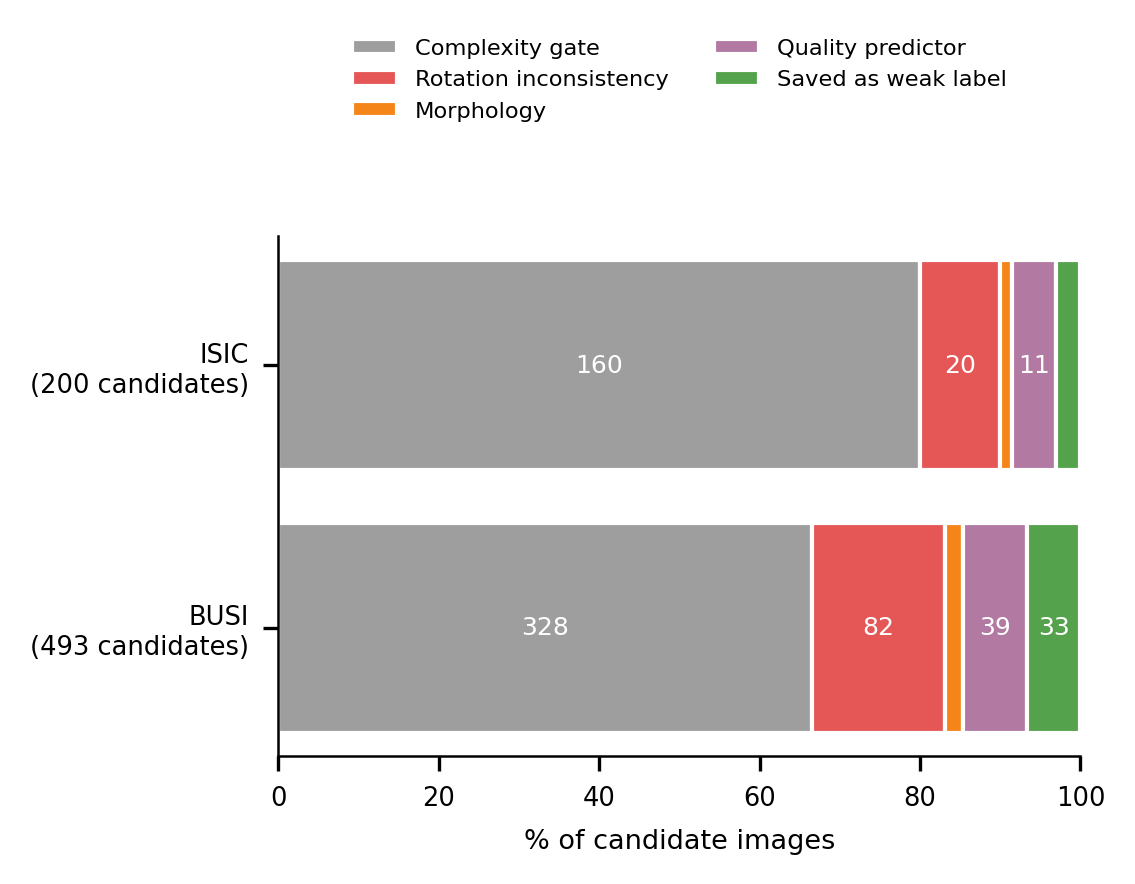
\includegraphics[width=0.88\columnwidth]{fig3_cascade.png}
\caption{Proportion of candidate images rejected at each cascade stage across BUSI and ISIC candidate pools.}
\label{fig:cascade}
\end{figure}

\subsection{Test-Time Augmentation (TTA) Evaluation}
Table~\ref{tab:tta} compiles all TTA measurements evaluated on the BUSI test set using `eval_tta.py`:
\begin{itemize}
    \item For the GS baseline, horizontal TTA increased Dice from 0.3846 to 0.3893 ($+0.0047$), and four-flip TTA reached 0.3904 ($+0.0058$).
    \item For the enhanced model (20 GS + 33 WL), four-flip TTA elevated Dice from 0.3966 to 0.4157 ($+0.0191$).
    \item For the 100 WL point-prompt model, horizontal TTA slightly shifted Dice from 0.5809 to 0.5822 ($+0.0013$).
    \item For the 100 WL box-prompt model, horizontal TTA attained a Dice of 0.5041 (IoU 0.4075).
\end{itemize}

\begin{table}[t]
\renewcommand{\arraystretch}{1.15}
\caption{BUSI Test-Time Augmentation Measurements (\texttt{eval\_tta.py}, 129 Images)}
\label{tab:tta}
\centering\footnotesize
\begin{tabular}{@{}llccc@{}}
\toprule
Model Checkpoint & TTA Mode & IoU & Dice & $\Delta$Dice \\
\midrule
\multirow{3}{*}{GS Baseline (20 GS)} & None & 0.4310 & 0.3846 & --- \\
 & Horizontal Flip & 0.4394 & 0.3893 & $+0.0047$ \\
 & Four-Way Flip & 0.4409 & 0.3904 & $+0.0058$ \\
\midrule
\multirow{3}{*}{Enhanced (20 GS + 33 WL, DW Loss)} & None & 0.3719 & 0.3966 & --- \\
 & Horizontal Flip & 0.3726 & 0.3986 & $+0.0020$ \\
 & Four-Way Flip & 0.3836 & 0.4157 & $+0.0191$ \\
\midrule
\multirow{2}{*}{100 WL Replicated Set (Points)} & None & 0.4907 & 0.5809 & --- \\
 & Horizontal Flip & 0.4972 & 0.5822 & $+0.0013$ \\
\midrule
100 WL Replicated Set (Box) & Horizontal Flip & 0.4075 & 0.5041 & n/a \\
\bottomrule
\end{tabular}
\end{table}

\subsection{Discrepancy Between Evaluation Scripts}
Table~\ref{tab:protocol} compares predictions on identical model checkpoints evaluated without augmentation across \texttt{eval.py} and \texttt{eval\_tta.py}.

\begin{table}[t]
\renewcommand{\arraystretch}{1.15}
\caption{Evaluation Script Discrepancy on Identical Model Checkpoints (BUSI)}
\label{tab:protocol}
\centering\footnotesize
\begin{tabular}{@{}lcccc@{}}
\toprule
 & \multicolumn{2}{c}{\texttt{eval.py} (Standard)} & \multicolumn{2}{c}{\texttt{eval\_tta.py} (Custom)} \\
\cmidrule(lr){2-3}\cmidrule(lr){4-5}
Evaluated Model & IoU & Dice & IoU & Dice \\
\midrule
GS Baseline (20 GS) & 0.3571 & 0.4209 & 0.4310 & 0.3846 \\
Enhanced Model (20 GS + 33 WL) & 0.2853 & 0.3905 & 0.3719 & 0.3966 \\
100 WL Set (Point Prompts) & 0.4732 & 0.6111 & 0.4907 & 0.5809 \\
\bottomrule
\end{tabular}
\end{table}

Under \texttt{eval\_tta.py}, IoU numerically exceeds Dice for the GS baseline (0.4310 vs.\ 0.3846), indicating that the script pools intersections and unions globally rather than computing per-image macro-averages (Section~\ref{subsec:metrics}). Crucially, relative model rankings invert between scripts: \texttt{eval.py} ranks the GS baseline above the enhanced model (0.4209 vs.\ 0.3905), whereas \texttt{eval\_tta.py} ranks the enhanced model higher (0.3966 vs.\ 0.3846).

\subsection{Contrastive Pretraining Loss Convergence}
Fig.~\ref{fig:simclr} plots the self-supervised SimCLR pretraining loss over epochs:
\begin{itemize}
    \item On BUSI, NT-Xent loss decreased from 0.7060 (epoch 1) to 0.5229 (epoch 15), reaching a minimum of 0.5020 at epoch 13.
    \item On ISIC, NT-Xent loss decreased from 4.1071 (epoch 1) to 3.6013 (epoch 5).
\end{itemize}
These trajectories verify that contrastive optimization functioned properly, although weights were not integrated into the segmentation training scripts.

\begin{figure}[t]
\centering
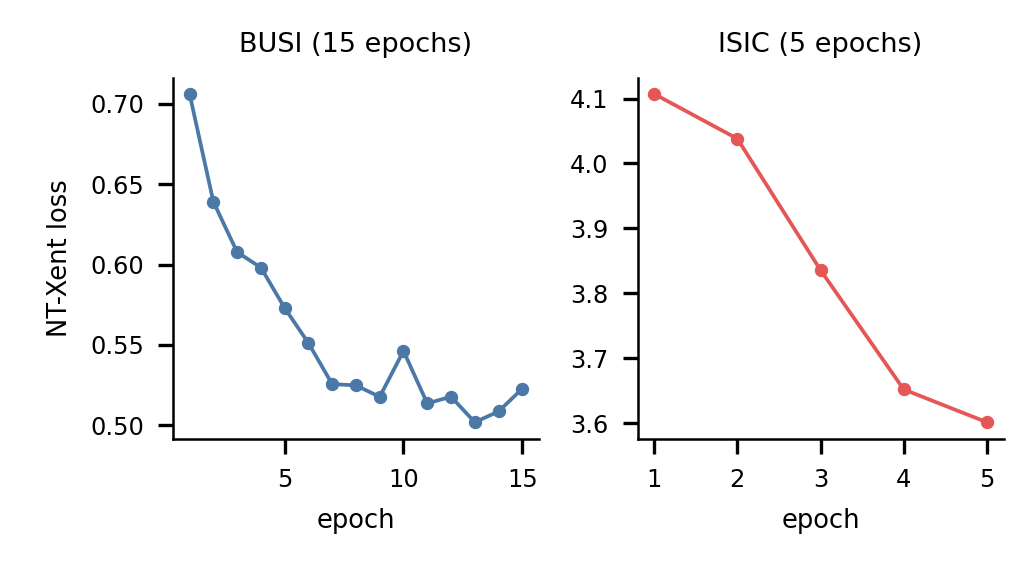
\includegraphics[width=0.88\columnwidth]{fig4_contrastive.png}
\caption{Self-supervised SimCLR pretraining loss (NT-Xent) convergence curves on unlabeled BUSI ultrasound (left) and ISIC dermoscopy (right) scans.}
\label{fig:simclr}
\end{figure}

\subsection{Weak-Label Volume and Test Performance}
Table~\ref{tab:count} summarizes weak-label volume against test Dice in \texttt{eval.py}. In both BUSI and ISIC, models with small numbers of cascade weak labels (33 and 6) did not improve over their GS baselines, whereas training on 100 weak labels yielded substantial performance boosts.

\begin{table}[t]
\renewcommand{\arraystretch}{1.15}
\caption{Weak-Label Training Volume vs.\ Test Dice Score (\texttt{eval.py})}
\label{tab:count}
\centering\footnotesize
\begin{tabular}{@{}llcc@{}}
\toprule
Dataset & Training Composition & Retained WL Count & Test Dice \\
\midrule
BUSI & 20 GS Baseline & 0 & 0.4209 \\
BUSI & 20 GS + Cascade WL, DW Loss & 33 & 0.3905 \\
BUSI & 25 GS + 100 WL (Box Prompts) & 100 & 0.4631 \\
BUSI & 25 GS + 100 WL (Point Prompts) & 100 & \textbf{0.6111} \\
\midrule
ISIC 2018 & 25 GS Baseline & 0 & 0.6779 \\
ISIC 2018 & 20 GS + Cascade WL, DW Loss & 6 & 0.6149 \\
\bottomrule
\end{tabular}
\end{table}

%==============================================================================
\section{Discussion}
\label{sec:discussion}

\subsection{Analysis of Empirical Findings}
Our investigation yields three primary observations:
\begin{enumerate}
    \item \textbf{Replication of Foundation Weak Supervision:} The core premise of Deshpande et al.~\cite{deshpande2024}—that promptable foundation models can generate useful pseudo-labels from scarce annotations—is confirmed on BUSI. When provided with 100 weak labels, test Dice increased from 0.4209 to 0.4631 (box prompts) and 0.6111 (point prompts).
    \item \textbf{Point Prompts Outperform Bounding Boxes:} Point prompts yielded a $+0.1480$ Dice advantage over bounding boxes on BUSI (0.6111 vs.\ 0.4631). In ultrasound imaging, where speckle noise obscures tumor boundaries, tight bounding boxes often introduce background tissue confusion, whereas tumor centroids combined with negative background points provide unambiguous localization.
    \item \textbf{The Volume vs.\ Purity Trade-off in Quality Control:} The five-stage cascade approved only 6.7\% of BUSI candidates and 3.0\% of ISIC candidates. Retraining on these small subsets reduced downstream performance (BUSI: 0.3905 vs.\ 0.4209 baseline; ISIC: 0.6149 vs.\ 0.6779 baseline). Deep convolutional networks exhibit inherent tolerance to modest label noise when trained on sufficiently diverse data~\cite{arpit2017}. Severely restricting weak-label volume starves the network of structural variability.
\end{enumerate}

\subsection{Hypotheses for Enhanced Model Performance}
Several factors explain why the cascade-retrained models scored lower in `eval.py`:
\begin{itemize}
    \item \emph{Selection Bias Toward Easy Examples:} The complexity gate and curriculum ordering preferentially approve scans the coarse network already handles well. The approved weak labels may thus offer little novel information.
    \item \emph{Sample Weight Halving:} The distance-weighted loss applies $\lambda = 0.5$ to weak labels, further reducing the effective supervisory signal of the 33 BUSI and 6 ISIC examples.
    \item \emph{Validation Noise in Checkpoint Selection:} Training held out only 5 clean GS images for validation, making checkpoint selection susceptible to stochastic fluctuations.
    \item \emph{Domain Mismatch in Gate Thresholds:} The morphological and complexity thresholds were calibrated on ultrasound. When applied to dermoscopy, they eliminated 97\% of candidates.
\end{itemize}

\subsection{Threats to Validity}
We identify the following limitations:
\begin{enumerate}
    \item \emph{Single Seed Execution:} Experiments were run with a single random seed (Seed 42); confidence intervals were not computed.
    \item \emph{Dataset Differences:} The ISIC experiments utilized ISIC 2018 Task 1 (518 test images) rather than the ISBI 2016 partition (379 test images) in~\cite{deshpande2024}.
    \item \emph{Unconnected Components:} SimCLR encoder weights and centroid coordinates were implemented and executed but not passed to downstream models.
    \item \emph{Evaluation Discrepancies:} \texttt{eval.py} and \texttt{eval\_tta.py} employ differing aggregation protocols, inverting baseline-versus-enhanced model rankings.
\end{enumerate}

%==============================================================================
\section{Conclusion}
\label{sec:conclusion}

In this work, we replicated the Auto-Generate-WLs medical weak-supervision pipeline on breast ultrasound (BUSI), achieving faithful agreement on box prompts (0.4631 replicated vs.\ 0.4661 published) and strong point-prompt performance (0.6111 replicated vs.\ 0.5302 published). We evaluated a five-stage quality verification cascade, distance-weighted loss retraining, self-supervised pretraining, and test-time augmentation. 

Our findings demonstrate that aggressive filtering thresholds can severely restrict weak-label volume, leading to lower segmentation performance than gold-standard baselines under standard evaluation scripts. Test-time augmentation yielded consistent within-script increments (+0.001 to +0.019 Dice), but evaluation protocol discrepancies must be standardized. Future work will focus on dataset-calibrated gate thresholds, end-to-end integration of pretrained encoders, and multi-seed significance testing.

%==============================================================================
\section*{Code and Data Availability}
All Jupyter notebooks, training scripts, and figure generation routines are available at: \url{https://github.com/VIJAYADITYARV/Medical-Foundation-Models-Research-}. Benchmark datasets are publicly available: BUSI~\cite{aldhabyani2020}, ISIC 2018~\cite{codella2019}, and SIIM-ACR Pneumothorax. The published reference code is hosted by the Stanford ML Group at \url{https://github.com/stanfordmlgroup/Auto-Generate-WLs}.

%==============================================================================
\appendices

\section{Audit of Experimental Status and Unverified Items}
\label{app:status}
\begin{itemize}
    \item \textbf{Unverified Experiments:} SIIM-ACR pneumothorax pipeline executed in code, but no numerical scores were output or saved. ISIC TTA ran without printing metric values.
    \item \textbf{Unconnected Code Elements:} Pretrained SimCLR encoder weights were stored on disk but not loaded by downstream segmentation training cells. Centroid point prompts were computed but \texttt{points=None} was passed in cascade MedSAM calls.
    \item \textbf{Evaluation Inconsistencies:} Disagreement between macro-averaged \texttt{eval.py} and global-pooled \texttt{eval\_tta.py} inverts relative model rankings.
\end{itemize}

\section{Notebook Cell Provenance of Reported Metrics}
\label{app:provenance}
Table~\ref{tab:provenance} indexes every empirical metric reported in this manuscript against the corresponding code cell in the provided Jupyter notebooks.

\begin{table}[h]
\renewcommand{\arraystretch}{1.15}
\caption{Notebook Cell Provenance for All Reported Empirical Metrics}
\label{tab:provenance}
\centering\footnotesize
\begin{tabular}{@{}llp{6.8cm}@{}}
\toprule
Dataset & Metric / Experiment & Notebook Cell Index \\
\midrule
BUSI & Data split sizes (647 total, 129 test, 25 GS, 493 unlabeled) & `BUSI_novelties.ipynb`, Cell 8 \\
BUSI & SimCLR contrastive pretraining loss (15 epochs) & `BUSI_novelties.ipynb`, Cell 11 \\
BUSI & GS Baseline evaluation (\texttt{eval.py}: IoU 0.3571, Dice 0.4209) & `BUSI_novelties.ipynb`, Cells 17, 37 \\
BUSI & Cascade skip logs and candidate attrition & `BUSI_novelties.ipynb`, Cell 29 \\
BUSI & Approved weak label count (33 WLs) & `BUSI_novelties.ipynb`, Cell 30 \\
BUSI & Enhanced model retraining (20 GS + 33 WL, DW Loss) & `BUSI_novelties.ipynb`, Cell 35 \\
BUSI & Enhanced model evaluation (\texttt{eval.py}: IoU 0.2853, Dice 0.3905) & `BUSI_novelties.ipynb`, Cell 37 \\
BUSI & Test-Time Augmentation evaluation (\texttt{eval\_tta.py}) & `BUSI_novelties.ipynb`, Cell 39 \\
BUSI & 100 WL Box Prompt evaluation (\texttt{eval.py}: IoU 0.3266, Dice 0.4631) & `BUSI_novelties.ipynb`, Cell 40 \\
BUSI & 100 WL Point Prompt evaluation (\texttt{eval.py}: IoU 0.4732, Dice 0.6111) & `BUSI_novelties.ipynb`, Cell 41 \\
\midrule
ISIC 2018 & Data split sizes (25 GS, 200 unlabeled, 518 test) & `ISIC_novelties_FINAL.ipynb`, Cell 9 \\
ISIC 2018 & SimCLR contrastive pretraining loss (5 epochs) & `ISIC_novelties_FINAL.ipynb`, Cell 11 \\
ISIC 2018 & GS Baseline evaluation (\texttt{eval.py}: IoU 0.6585, Dice 0.6779) & `ISIC_novelties_FINAL.ipynb`, Cells 17, 36 \\
ISIC 2018 & Cascade skip logs and approved count (6 WLs) & `ISIC_novelties_FINAL.ipynb`, Cell 29 \\
ISIC 2018 & Enhanced model retraining (20 GS + 6 WL, DW Loss) & `ISIC_novelties_FINAL.ipynb`, Cell 34 \\
ISIC 2018 & Enhanced model evaluation (\texttt{eval.py}: IoU 0.5868, Dice 0.6149) & `ISIC_novelties_FINAL.ipynb`, Cell 36 \\
\midrule
SIIM-ACR & Pipeline implementation & `CANDIDPTX_novelties4.ipynb`, Cells 8--38 \\
\bottomrule
\end{tabular}
\end{table}

%==============================================================================
\begin{thebibliography}{30}

\bibitem{tajbakhsh2020}
N.~Tajbakhsh, L.~Jeyaseelan, Q.~Li, J.~N.~Chiang, Z.~Wu, and X.~Ding, ``Embracing imperfect datasets: A review of deep learning solutions for medical image segmentation,'' \emph{Med.\ Image Anal.}, vol.~63, p.~101693, 2020.

\bibitem{zhou2018}
Z.~Zhou, M.~M.~R.~Siddiquee, N.~Tajbakhsh, and J.~Liang, ``UNet++: A nested U-Net architecture for medical image segmentation,'' in \emph{DLMIA/ML-CDS}, 2018, pp.~3--11.

\bibitem{kirillov2023}
A.~Kirillov \emph{et al.}, ``Segment anything,'' \emph{arXiv:2304.02643}, 2023.

\bibitem{ma2023medsam}
J.~Ma, Y.~He, F.~Li, L.~Han, C.~You, and B.~Wang, ``Segment anything in medical images,'' \emph{Nature Communications}, vol.~15, no.~1, p.~654, 2024.

\bibitem{deshpande2024}
T.~Deshpande, E.~Prakash, E.~G.~Ross, C.~Langlotz, A.~Ng, and J.~M.~J.~Valanarasu, ``Auto-generating weak labels for real \& synthetic data to improve label-scarce medical image segmentation,'' in \emph{Proc.\ Medical Imaging with Deep Learning (MIDL)}, \emph{PMLR}, vol.~227, 2024, pp.~1--15.

\bibitem{deoliveira2023}
C.~M.~de~Oliveira \emph{et al.}, ``Zero-shot performance of the segment anything model (SAM) in 2D medical imaging: A comprehensive evaluation and practical guidelines,'' \emph{arXiv:2305.00109}, 2023.

\bibitem{he2023sam}
S.~He \emph{et al.}, ``Computer-vision benchmark Segment-Anything Model (SAM) in medical images: Accuracy in 12 datasets,'' \emph{arXiv:2304.09148}, 2023.

\bibitem{lee2013}
D.-H.~Lee, ``Pseudo-label: The simple and efficient semi-supervised learning method for deep neural networks,'' in \emph{ICML Workshop on Challenges in Representation Learning}, 2013.

\bibitem{tarvainen2017}
A.~Tarvainen and H.~Valpola, ``Mean teachers are better role models: Weight-averaged consistency targets improve semi-supervised deep learning results,'' in \emph{Proc.\ NeurIPS}, 2017.

\bibitem{yu2019}
L.~Yu, S.~Wang, X.~Li, C.-W.~Fu, and P.-A.~Heng, ``Uncertainty-aware self-ensembling model for semi-supervised 3D left atrium segmentation,'' in \emph{Proc.\ MICCAI}, 2019.

\bibitem{chen2021cps}
X.~Chen, Y.~Yuan, G.~Zeng, and J.~Wang, ``Semi-supervised semantic segmentation with cross pseudo supervision,'' in \emph{Proc.\ CVPR}, 2021.

\bibitem{chen2020simclr}
T.~Chen, S.~Kornblith, M.~Norouzi, and G.~Hinton, ``A simple framework for contrastive learning of visual representations,'' in \emph{Proc.\ ICML}, 2020.

\bibitem{chaitanya2020}
K.~Chaitanya, E.~Erdil, N.~Karani, and E.~Konukoglu, ``Contrastive learning of global and local features for medical image segmentation with limited annotations,'' in \emph{Proc.\ NeurIPS}, 2020.

\bibitem{butoi2023}
V.~I.~Butoi \emph{et al.}, ``UniverSeg: Universal medical image segmentation,'' in \emph{Proc.\ ICCV}, 2023.

\bibitem{lin2023}
X.~Lin \emph{et al.}, ``SAMUS: Adapting segment anything model for clinically-friendly and generalizable ultrasound image segmentation,'' \emph{arXiv:2309.06824}, 2023.

\bibitem{shin2023}
D.~Shin, B.~Kim, and S.~Baek, ``CEmb-SAM: Segment anything model with condition embedding for joint learning from heterogeneous datasets,'' in \emph{MICCAI Workshops}, 2023, pp.~275--284.

\bibitem{chen2023}
C.~Chen \emph{et al.}, ``MA-SAM: Modality-agnostic SAM adaptation for 3D medical image segmentation,'' \emph{Medical Image Analysis}, vol.~97, p.~103280, 2024.

\bibitem{pandey2023}
S.~Pandey, K.~Chen, and E.~B.~Dam, ``Comprehensive multimodal segmentation in medical imaging: Combining YOLOv8 with SAM and HQ-SAM models,'' in \emph{Proc.\ ICCV Workshops}, 2023, pp.~2584--2590.

\bibitem{wu2024}
Q.~Wu, Y.~Zhang, and M.~Elbatel, ``Self-prompting large vision models for few-shot medical image segmentation,'' in \emph{Domain Adaptation and Representation Transfer}, 2024, pp.~156--167.

\bibitem{lei2023}
W.~Lei, X.~Wei, X.~Zhang, K.~Li, and S.~Zhang, ``MedLSAM: Localize and segment anything model for 3D CT images,'' \emph{arXiv:2306.14752}, 2023.

\bibitem{arpit2017}
D.~Arpit \emph{et al.}, ``A closer look at memorization in deep networks,'' in \emph{Proc.\ ICML}, 2017.

\bibitem{wang2019}
G.~Wang, W.~Li, M.~Aertsen, J.~Deprest, S.~Ourselin, and T.~Vercauteren, ``Aleatoric uncertainty estimation with test-time augmentation for medical image segmentation with convolutional neural networks,'' \emph{Neurocomputing}, vol.~338, pp.~34--45, 2019.

\bibitem{aldhabyani2020}
W.~Al-Dhabyani, M.~Gomaa, H.~Khaled, and A.~Fahmy, ``Dataset of breast ultrasound images,'' \emph{Data in Brief}, vol.~28, p.~104863, 2020.

\bibitem{codella2019}
N.~Codella \emph{et al.}, ``Skin lesion analysis toward melanoma detection 2018: A challenge hosted by the International Skin Imaging Collaboration (ISIC),'' \emph{arXiv:1902.03368}, 2019.

\bibitem{gutman2016}
D.~Gutman \emph{et al.}, ``Skin lesion analysis toward melanoma detection: A challenge at ISBI 2016, hosted by the International Skin Imaging Collaboration (ISIC),'' \emph{arXiv:1605.01397}, 2016.

\bibitem{feng2021}
S.-Y.~Feng \emph{et al.}, ``Curation of the CANDID-PTX dataset with free-text reports,'' \emph{Radiology: Artificial Intelligence}, vol.~3, no.~6, p.~e210136, 2021.

\bibitem{ho2020}
J.~Ho, A.~Jain, and P.~Abbeel, ``Denoising diffusion probabilistic models,'' in \emph{Proc.\ NeurIPS}, 2020.

\bibitem{wolleb2021}
J.~Wolleb, R.~Sandk{\"u}hler, F.~Bieder, P.~Valmaggia, and P.~C.~Cattin, ``Diffusion models for implicit image segmentation ensembles,'' \emph{arXiv:2112.03145}, 2021.

\bibitem{fraz2012}
M.~M.~Fraz \emph{et al.}, ``An ensemble classification-based approach applied to retinal blood vessel segmentation,'' \emph{IEEE Trans.\ Biomed.\ Eng.}, vol.~59, no.~9, pp.~2538--2548, 2012.

\end{thebibliography}

\end{document}
